\documentclass{report}
\usepackage[fontsize=13pt]{scrextend}

\usepackage{my_lab}

\begin{document}

\graphicspath{{figures}}

\LabTitle{3.2.6}{Изучение гальванометра}

\begin{document}
\textbf{Цель работы}:
Изучение работы высокочувствительного зеркального гальванометра
магнитоэлектрической системы в режимах измерения постоянного тока и
электрического заряда.

\textbf{В работе используются:}:
\begin{enumerate}
	\item зеркальный гальванометр с осветителем и шкалой
	\item источник постоянного напряжения
	\item делитель напряжения
	\item магазин сопротивлений
	\item эталонный конденсатор
	\item вольтметр
	\item переключатель
	\item ключи
	\item линейка
\end{enumerate}

\section{Краткая Теория}

\textit{Баллистический гальванометр} -- электроизмерительный прибор
магнитоэлектрической системы, отличающийся высокой чувствительностью к току и
сравнительно большим периодом свободных колебаний. \par
На помещённую в магнитное поле обтекаемую током рамку гальванометра действуют
момент закрученной нити, момент магнитных сил и тормозящий момент (зависит от
сил сопротивления воздуха и от вихревых токов). Учитывая все эти моменты,
уравнение движения рамки принимает вид
\begin{center}
	$\ddot \varphi + 2 \gamma \dot \varphi + \omega_0^2\varphi = KI $,
\end{center}
где $\gamma$ -- коэффициент затухания подвижной системы гальванометра, $\omega_0$ -- собственная частота колебаний рамки

Динамическая постоянная гальванометра определяется при пропускании через рамку постоянного тока:
\begin{center}
	$C_I = \frac{I}{\varphi} = \frac{D}{BSN}$,
\end{center}
где $B$ - индукция магнитного поля в рамке, $S$ - площадь одного витка рамки, $D$ - модуль кручения нити. \par
При пропускании коротких импульсов тока через баллистический гальванометр
начальная скорость движения рамки пропорциональна электрическому заряду,
прошедшему через рамку за всё время импульса. Отношение баллистических
постоянных в критическом и свободном режимах равно $e$.

\section{Экспериментальная установка}
\subsection{Определение динамической постоянной}
\begin{figure}[h]
	\centering
	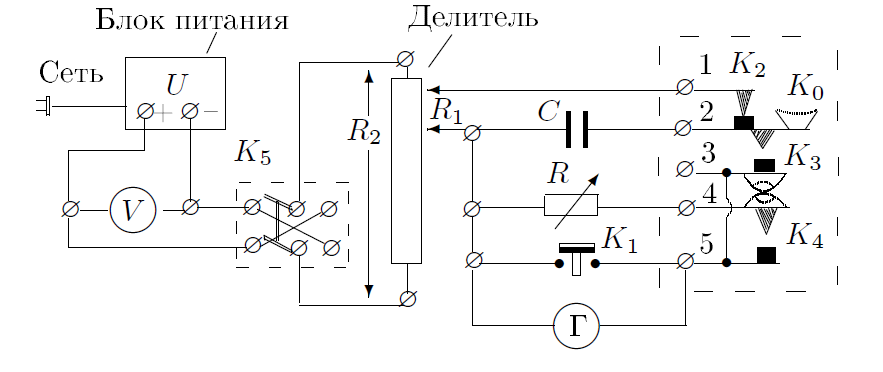
\includegraphics[width=10cm]{fig1.PNG}
	\caption{Схема установки для работы гальванометра в стационарном режиме}
	\label{fig:vac}
\end{figure}
Постоянное напряжение $U = 1,5$В снимается с блока питания и измеряется
вольтметром $V$. Ключ $K_3$ позволяет менять величину тока через гальванометр
Г, делитель напряжения - менять величину тока в широких пределах. Ключ $K_2$
служит для включения гальванометра, кнопка $K_1$ -- для его успокоения. Магазин
сопротивлений $R$ позволяет менять режим работы гальванометра от колебательного
до апериодического. \par
При малых $R_1$ сила тока, протекающего через гальванометр, может быть вычислена по формуле
\begin{equation}
	I = U_0 \frac{R_1}{R_2} \frac{1}{R + R_0}.
\end{equation}
Динамическую постоянную вычисли по формуле
\begin{equation}
	C_I = \frac{2aI}{x},
\end{equation}
где $a$ - расстояние от шкалы до зеркальца.

\subsection{Определение критического сопротивления гальванометра}
Выполняется с помощью той же цепи, что и на рис. 1. При больших $R$ движение
рамки имеет колебательный характер, с уменьшением $R$ затухание увеличивается,
и колебательный режим переходит в апериодический. \par
Найдём логарифмический декремент затухания колебаний рамки  $\Theta$.
\begin{equation}
	\Theta = ln\frac{x_n}{x_{n+1}} = \gamma T = \frac{2\pi \gamma}{\sqrt{\omega_0^2 - \gamma^2}} = \frac{2\pi R_3}{\sqrt{(R_0 + R)^2 - R_3^2}}
\end{equation}

Рассчитаем критическое сопротивление по графику в координатах $X = (R_0^2 + R)$, $Y = 1/\Theta^2$
\begin{equation}
	R_{c_r} = \frac{1}{2\pi}\sqrt{\frac{\triangle X}{\triangle Y}} - R_0
\end{equation}

\subsection{Определение баллистической постоянной и критического сопротивления гальванометра, работающего в баллистическом режиме}

Для изучения работы гальванометра в режиме измерения заряда используется схема, представленная на рис. 2.

\begin{figure}[h]
	\centering
	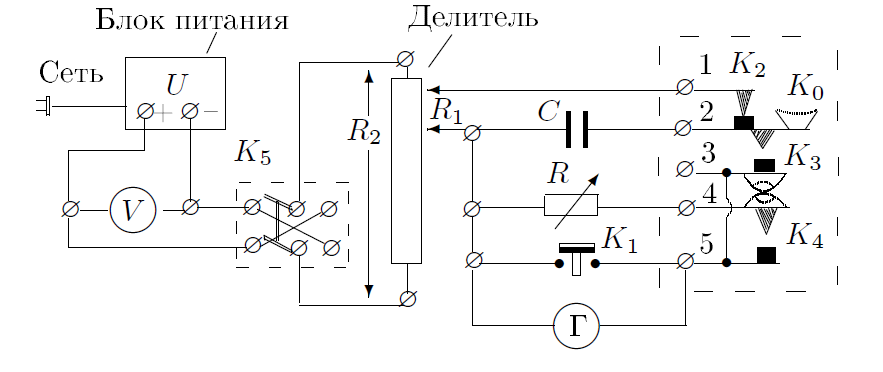
\includegraphics[width=10cm]{fig1.PNG}
	\caption{Схема установки для определения баллистической постоянной}
	\label{fig:vac}
\end{figure}

При нормальном положении кнопки $K_0$ конденсатор $C$ заряжается до напряжения
\begin{center}
	$U_c = \frac{R_1}{R_2}U_0$
\end{center}
Заряд конденсатора равен
\begin{center}
	$q = \frac{R_1}{R_2}U_0 C$
\end{center}
При нажатии на ключ $K_0$ конденсатор отключается от источника постоянного
напряжения и подключается к гальванометру. К моменту замыкания ключа $K_4$ весь
заряд успевает пройти через гальванометр, рамка получает начальную скорость.
Баллистическая постоянная гальванометра определяется при критическом
сопротивлении
\begin{equation}
	C_{Q_{c_r}} = \frac{q}{\varphi_{max cr}} = 2a\frac{R_1}{R_2} \frac{U_0 C}{l_{max cr}}
\end{equation}

\section{Ход работы}
\begin{table}[H]
	\centering
	\begin{tabular}{|l|l|}
		\hline
		$a, \m$ & $1 \pm 0.02$ \\
		\hline
	\end{tabular}
\end{table}
\subsection{Динамическая постоянная}
\begin{equation*}
	I = \frac{C_I}{2a} x
\end{equation*}
$C_I$ - динамическая постоянная гальванометра. \\
$I = \frac{R_1}{R_2} \frac{U_0}{R + R_0}$

\begin{figure}[H]
	\centering
	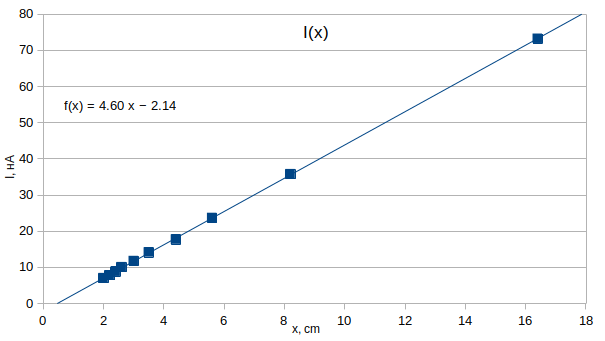
\includegraphics[width=0.9\linewidth]{figures/g1.png}
\end{figure}

\begin{table}[H]
	\centering
	\begin{tabular}{|l|l|l|}
		\hline
		$R, \kilo\Ohm$ & $x, \cm$ & $I, \nano A$ \\
		\hline
		99             & 2        & 7            \\
		89             & 2.2      & 8            \\
		79             & 2.4      & 9            \\
		69             & 2.6      & 10           \\
		59             & 3        & 12           \\
		49             & 3.5      & 14           \\
		39             & 4.4      & 18           \\
		29             & 5.6      & 24           \\
		19             & 8.2      & 36           \\
		9              & 16.4     & 73           \\
		\hline
	\end{tabular}
\end{table}

\begin{equation*}
	C_I = (9.2 \pm 0.1) \cdot 10^{-10} \frac{A}{\mm / \m}
\end{equation*}

\begin{equation*}
	S_I = \frac{1}{C_I} = (11.0 \pm 0.2) \cdot 10^{8} \frac{\mm / \m}{A}
\end{equation*}

\subsection{Критическое сопротивление}
$\theta_0 = \frac{1}{3} \sum{\ln\frac{x_n}{x_{n+1}}}$
\begin{equation*}
	\theta_0 \approx 0.3
\end{equation*}
\begin{table}[H]
	\centering
	\begin{tabular}{|l|l|l|l|l|l|}
		\hline
		N  & $R, \kilo\Ohm$ & $x_n, \cm$ & $x_{n+k}, \cm$ & $\theta$ & $R_{\text{кр}}, \Ohm$ \\
		\hline
		1  & 24             & 5.9        & 0.8            & 2.0      & 7.89                  \\
		2  & 28             & 11.1       & 1.7            & 1.9      & 8.62                  \\
		3  & 32             & 10.6       & 1.6            & 1.7      & 8.81                  \\
		4  & 36             & 10.3       & 2.4            & 1.5      & 8.31                  \\
		5  & 40             & 10.2       & 2.7            & 1.3      & 8.84                  \\
		6  & 44             & 9.8        & 3.0            & 1.2      & 8.69                  \\
		7  & 48             & 9.8        & 3.2            & 1.1      & 7.96                  \\
		8  & 56             & 14.4       & 5.3            & 1.0      & 8.33                  \\
		9  & 64             & 13.0       & 5.2            & 0.9      & 8.76                  \\
		10 & 72             & 12.0       & 5.2            & 0.8      & 9.02                  \\
		11 & 80             & 11.8       & 5.5            & 0.7      & 9.16                  \\
		\hline
	\end{tabular}
\end{table}

\begin{equation*}
	\avrg{R_{\text{кр}}} = (8.6 \pm 0.1) \kilo\Ohm
\end{equation*}

\subsection{Баллистическая постоянная}

\begin{table}[H]
	\centering
	\begin{tabular}{|l|l|}
		\hline
		$R, \kilo\Ohm$ & $x_{\max}, \cm$ \\
		\hline
		50             & 16.0            \\
		45             & 15.8            \\
		40             & 15.5            \\
		35             & 15.0            \\
		30             & 14.9            \\
		25             & 14.5            \\
		20             & 13.5            \\
		15             & 13.0            \\
		10             & 11.0            \\
		5              & 7.5             \\
		4              & 6.3             \\
		2              & 3.1             \\
		\hline
	\end{tabular}
\end{table}

\begin{gather*}
	x_{0} = 17.5 \cm \\
	x_1 = x_0 \cdot e^{\frac{\theta_0}{4}} \approx 19 \cm \\
	x_e = \frac{x_0}{e} \approx 7 \cm
\end{gather*}

\begin{gather*}
    \frac{1}{R + R_0} (x_e) \approx 20 \cdot 10^{-5} \Cm \implies \\
    R \approx 4.5 \kilo\Ohm
\end{gather*}

\section{Вывод}
Итак, в этой работе мы изучили работу гальванометра в трех режимах:
стационарном, свободных колебаний и баллистическом. Мы измерили критическое
сопротивление контура $ R_{кр} $ тремя способами, а также нашли динамическую и
баллистическую постоянную установки. 

\end{document}
